\documentclass[presentation,sansserif]{beamer}
\usefonttheme[onlymath]{serif}
%\renewcommand\mathfamilydefault{ppl}
%\usetheme{Warsaw}
%\usecolortheme{beetle}
\usepackage {mathpazo}
\usepackage{graphicx}
\usepackage{blindtext}
\usepackage{xfrac}

\title[Developing pop-gen models for polyploids]{Developing models for genotype uncertainty, inbreeding, and allelic inheritance in non-model polyploids}
\author[Blischak \textit{et al}.]{Paul Blischak$^1$ :: Laura Kubatko$^{1,2}$ :: Andrea Wolfe$^1$}

%\institute[OSU]{{\small Dept. of Evolution, Ecology\\ and Organismal Biology\\[0.15in] \textsc{The Ohio State University}}}

\date{}

\definecolor{itemcol}{RGB}{0,128,255}
\definecolor{back}{RGB}{1,22,39}
\definecolor{alert}{RGB}{255,0,81}
\definecolor{yell}{RGB}{255,222,0}
\setbeamercolor{alerted text}{fg=alert}
\setbeamercolor{section in toc}{fg=black, bg=black}
\setbeamercolor{item}{fg=itemcol,bg=itemcol}
\setbeamercolor{structure}{fg=itemcol!95!black}
\setbeamercolor{background canvas}{bg=white!15!black}
%\setbeamercolor{background canvas}{bg=back}
\setbeamercolor{normal text}{fg=white!95!black, bg=white!95!black}
\setbeamercolor{math text}{fg=white, bg=white}
%\setbeamertemplate{items}[square]
%\setbeamertemplate{items in toc shaded}[square]
%\setbeamertemplate{items in toc}[square]

\newcommand{\inline}[1]{\fcolorbox{white!15!black}{white!20!black}{\texttt{#1}}}

\setbeamertemplate{navigation symbols}{% 
%\insertslidenavigationsymbol 
%\insertframenavigationsymbol 
%\insertsubsectionnavigationsymbol 
%\insertsectionnavigationsymbol 
%\insertdocnavigationsymbol 
%\insertbackfindforwardnavigationsymbol \hspace{1em}%
 \usebeamerfont{footline} \insertframenumber/\inserttotalframenumber% 
 }

\begin{document}

\beamertemplatenavigationsymbolsempty

\begin{frame}[plain]
	\vspace{-1.2in}
	\titlepage
	
	\vspace{-1.2in}
	\begin{center}
	
		{\footnotesize Ohio State University 	
		\vspace{0.05in}
		
		$^1$Department of EEOB :: $^2$Department of Statistics
		}		
	\end{center}
	\vspace{-0.2in}
		
\end{frame}


\begin{frame}[t]{The world of polyploidy}
  \vspace{0.3in}
  \pause
  
  \textbf{More than just plants}.
  \vspace{0.3in}
  \pause
  
  ...but mostly plants.
  \vspace{0.3in}
  \pause
  
  Common in several lineages of fish (sturgeon and salmon), amphibians (salamanders), and fungi (yeast).

\end{frame}

\begin{frame}[t]{The world of polyploidy}
\framesubtitle{Types of polyploids}

	\onslide<2->{\textbf{Autopolyploids}:}

	\begin{center}
		\onslide<3->{\includegraphics[width=0.5\textwidth]{eps/autopolyploid-formation}}
	\end{center}
	
	\onslide<2->{\textbf{Allopolyploids}:}
	
	\begin{center}
		\onslide<4->{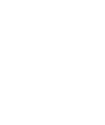
\includegraphics[width=0.5\textwidth]{eps/allopolyploid-formation}}
	\end{center}

\end{frame}

\begin{frame}[t]{Non-model polyploids}
  \vspace{0.3in}

  The majority of polyploid organisms have little to no genomic resources available.
  \vspace{0.3in}
  \pause
  
  There is a need to 
  

  
  \onslide<4->{We need methods }

\end{frame}

\begin{frame}[t]{Polyploid pop-gen}
  \framesubtitle{Challenges}
  
  \vspace{0.1in}
  The difficulties of making population genetic inferences in polyploids present themselves at two broad levels:
  \vspace{0.2in}
  %\pause

	\begin{enumerate}
		\onslide<2->{\item \textbf{Allelic dosage}: difficult to determine the number of allele copies.}
		\vspace{0.1in}
		
		\begin{itemize}
			\onslide<3>{\item Ex: Two alleles are present in a tetraploid. Is the genotype ABBB, AABB, or AAAB?}
		\end{itemize}
		\vspace{0.2in}
		\pause

		\onslide<4->{\item \textbf{Allelic inheritance}: how do chromosomes pair during meiosis? Do subgenomes interact?}
	\end{enumerate}
	
\end{frame}

\begin{frame}[t]{Dealing with allelic dosage}
	\pause
	\vspace{0.1in}
	Account for genotype uncertainty...
	\vspace{0.2in}

	\begin{itemize}
	\setlength\itemsep{0.2in}
		\item Our previous model used a hierarchical setup for high throughput sequencing (HTS) data, genotypes, and allele frequencies.
		\vspace{0.1in}
		\pause

		\item Joint inference on genotypes and frequencies using Gibbs sampling (implemented in the R package \textbf{polyfreqs}).
		\vspace{0.1in}
		\pause

		\item Turns out there is a better way \pause $\rightarrow$ (1) don't sample genotypes\pause, (2) don't use Gibbs sampling (too expensive).
		\vspace{0.1in}

	\end{itemize}

\end{frame}

\begin{frame}[t]{Dealing with allelic dosage}
	\framesubtitle{Genotype likelihoods}

	Instead, we pre-compute genotype likelihoods (e.g., using GATK) and directly calculate the sum over genotypes.
	\vspace{0.2in}
	\pause
	
	$D$ -- HTS data (reads and error values)
	
	$m$ -- ploidy-level
	
	$G$ -- genotype $(0,\dots,m)$
	
	$p$ -- allele frequency
	

	\pause
	\begin{equation*}
		\mathcal{L}(G) = P(D|G).
	\end{equation*}
	\vspace{-0.1in}
	
	\begin{equation*}
		\mathcal{L}(p) = P(D|p) = \sum_G P(D|G)P(G|p),
	\end{equation*}
	\vspace{-0.2in}
	\pause
	
	\begin{equation*}
		= \sum_G \mathcal{L}(G)P(G|p).
	\end{equation*}

\end{frame}

\begin{frame}[t]{Assumptions}

  \begin{enumerate}
    \setlength\itemsep{0.25in}
    \item Hardy-Weinberg equilibrium (HWE).
    \item Loci are unlinked and independent.
    \item Genotypes are drawn from a single pool of alleles $=$ allelic inheritance pattern for autopolyploid.
  \end{enumerate}
  \vspace{0.25in}
  \pause

Mixed mating systems and double reduction can make HWE a poor assumption in autopolyploids \pause $\rightarrow$ inbreeding and increased homozygosity.
\vspace{0.25in}
\pause

Allopolyploids inherit two($+$) sets of chromosomes with different ancestries \pause $\rightarrow$ assuming draws from a single allele pool does not reflect their hybrid origin.

\end{frame}

\begin{frame}[t]{Dealing with inheritance patterns}

  $F$-models for genetic correlations.

\end{frame}

\begin{frame}[t]{A disequilibrium model for autopolyploids}

  In most models, $P(G|p)$ is binomially distributed, implying that genotypes are drawn in HW proportions.
  \vspace{0.3in}
  \pause
  
  To relax this, we use a different probability distribution for genotypes: the beta-binomial.
  \vspace{0.3in}
  \pause
  
  Using an additional parameter, $\phi$, the probability distribution for genotypes becomes
  \vspace{0.1in}
  
  \begin{equation}
    P(G=a|p,\phi) = \frac{\mathcal{B}(a + p\phi, m - a + (1-p)\phi)}{\mathcal{B}(p\phi, (1-p)\phi)}.
  \end{equation}
  \vspace{0.2in}
  \pause
  

Here, $\mathcal{B}()$ is the beta function, and $\phi$ is related to the inbreeding coefficient as $F = \sfrac{1}{(1+\phi)}$.

\end{frame}

{ \setbeamercolor{background canvas}{bg=white!20!black} \setbeamercolor{math text}{bg=itemcol, fg=itemcol}
\begin{frame}[c,plain]{The effect of $F$}

  \begin{center}
    \frame{\includegraphics[width=0.9\textwidth]{pdf/genotype-freqs-diseq}}
  \end{center}
  
\end{frame}

}

{ \setbeamercolor{background canvas}{bg=white!20!black}
\begin{frame}[c,plain]{Disequilibrium model}
	\framesubtitle{\hspace{15pt}}
	\begin{center}
		\frame{\includegraphics[width=\textwidth]{pdf/freq-phi-lik-surf2}}
	\end{center}
\end{frame}
}

\begin{frame}[t]{A subgenome model for allopolyploids}
\pause

Consider the simple case of two sets of chromosomes with different ancestry that do not interact (no homoeologous recombination).
\vspace{0.3in}
\pause

We use a commonly employed $F$-model for correlated allele frequencies in the two subgenomes: divergence from a common ancestor with drift.
\vspace{0.3in}
\pause


$\pi$ -- ancestral allele frequency\\
$\theta$ -- drift [related to $F_{st} = 1/(1+\theta)$] \\
$p_1,p_2$ -- allele frequencies in subgenome one and two\\
\vspace{0.3in}
\pause

\begin{equation}
p_i|\pi,\theta \sim \text{beta}(\pi\theta,(1-\pi)\theta), \quad \text{for } i=1,2.
\end{equation}

\end{frame}

\begin{frame}[t]{A subgenome model for allopolyploids}

Genotypes are now a mixture of draws from the two subgenomes, each with a potentially different allele frequency.
\vspace{0.25in}
\pause

Given the ploidy of the two subgenomes ($m_1$,$m_2$), the genotype can be modeled as a sum of two binomially distributed random variable.
\vspace{0.25in}
\pause

This is a special case of the poisson-binomial distribution, which models binomial experiments when the probability of success is not the same for each trial.
\pause

\begin{align}
P(G&=a|p_1,p_2,m_1,m_2) \nonumber \\[0.05in]
&= P(G=i|p_1,m_1) + P(G=j|p_2,m_2), \nonumber \\[0.05in]
&\text{ for } i=1,\dots,m_1; \; j=1,\ldots,m_2; \; i+j=a.
\end{align}

\end{frame}

{ \setbeamercolor{background canvas}{bg=white!20!black} %\setbeamercolor{math text}{fg=itemcol, bg=itemcol}
\begin{frame}[c,plain]{Subgenome model}
	\framesubtitle{$F_{st}=0.1$}
	\begin{center}
		\frame{\includegraphics[width=\textwidth]{pdf/freq1-freq2-lik-surf1}}
	\end{center}
\end{frame}
}

{ \setbeamercolor{background canvas}{bg=white!20!black} %\setbeamercolor{math text}{fg=itemcol, bg=itemcol}
\begin{frame}[c,plain]{Subgenome model}
	\framesubtitle{$F_{st}=0.5,\, \pi=0.475,\, p_1=0.962,\, p_2=0.343$}
	\begin{center}
		\frame{\includegraphics[width=\textwidth]{pdf/freqs1-freqs2-bad-lik-surf1}}
	\end{center}
\end{frame}
}

{ \setbeamercolor{background canvas}{bg=white!20!black} %\setbeamercolor{math text}{fg=itemcol, bg=itemcol}
\begin{frame}[c,plain]{Subgenome model}
	\framesubtitle{$F_{st}=0.5,\, \pi=0.922,\, p_1=0.999,\, p_2=0.414$}
	\begin{center}
		\frame{\includegraphics[width=\textwidth]{pdf/freqs1-freqs2-bad-lik-surf3}}
	\end{center}
\end{frame}
}


\begin{frame}[t]{Conclusions and future directions}
	\pause
	\fontsize{10pt}{10}\selectfont
	\begin{enumerate}
		\item{Conclusions:}
		\setlength\itemsep{0.1in}
		\begin{itemize}
			\setlength\itemsep{0.1in}
			\item $F$-models have great potential for helping make inferences in non-model polyploids.
			\vspace{0.2in}
		\end{itemize}
		\pause
		\item{Future directions:}
		\setlength\itemsep{0.1in}
		\begin{itemize}
		\setlength\itemsep{0.1in}
			\item Include parental data in allopolyploid model if available and develop a model selection framework for testing allopolyploid parentage. \pause
			\item Currently developing software 
		\end{itemize}
	\end{enumerate}

\end{frame}

\begin{frame}[t,plain]{Code availability}
	\fontsize{10pt}{10}\selectfont
	\begin{itemize}
	\setlength\itemsep{0.2in}

		\item Presentation slides are on fig\textbf{share}.
		
		\item \LaTeX{} source code is on GitHub:\\[0.05in] \url{https://github.com/pblischak/evolution2016}.
		
		\item R package (\textbf{ppgtkR}) and code for simulating data under the different models, as well as calculating and plotting the log-likelihood surface, are also on GitHub: \\[0.05in] \url{https://github.com/pblischak/ppgtkR}
		
	\end{itemize}
	\vspace{0.15in}

	{\Large \alert{All these links are in the GitHub repository for this presentation: \textbf{pblischak/evolution2016}.}}

	\hfill {\tiny \#openscience}
\end{frame}

\begin{frame}[t,plain]{Acknowledgments}
  \vspace{0.2in}

  \begin{itemize}
    \setlength\itemsep{0.3in}
    \item John Novembre, Xin He, Matthew Stephens, and their lab members for the opportunity to present at U. of Chicago (and to John Blischak for organizing the visit).
    \item My labmates in the Wolfe and Kubatko labs.
    \item National Science Foundation for funding the larger project that includes the development of the models presented here.
  \end{itemize}

\end{frame}

\begin{frame}[c,plain]{}
	\begin{center}
		{\Huge Thanks!}\\
		\vspace{0.5in}
		{\LARGE Questions?}
	\end{center}
\end{frame}

\end{document}
